\documentclass{article}

\begin{document}
\chapter{Implementation}

PLSI is designed to be portable to multiple technologies, CAD tool vendors, and
processor generators.  As such it has a modular system of addons that can be
mixed and matched in order to produce a chip.  Users are expected to define the
following variables, which will be used to control the flow:

\begin{itemize}
\item \texttt{CORE\_GENERATOR}
\item \texttt{SOC\_GENERATOR}
\item \texttt{TECHNOLOGY}
\item \texttt{SYNTHESIS\_TOOL}
\item \texttt{PAR\_TOOL}
\item \texttt{FORMAL\_TOOL}
\item \texttt{SIGNOFF\_POWER\_TOOL}
\item \texttt{SIMULATOR}
\end{itemize}

It is also possible to pass configuration information to each step in the flow
by setting the following variables

\begin{itemize}
\item \texttt{CORE\_CONFIG}
\item \texttt{CORE\_SIM\_CONFIG}
\item \texttt{SOC\_CONFIG}
\item \texttt{MAP\_CONFIG}
\end{itemize}

A top-level Makefile sequences the entire chip build; which includes running
all the CAD tools, testing the designs after every tool is run, and
interpreting the results.  A high-level overview of the PLSI flow can be seen
in Figure~\ref{impl:plsi-flow}.

\begin{figure}
\begin{center}
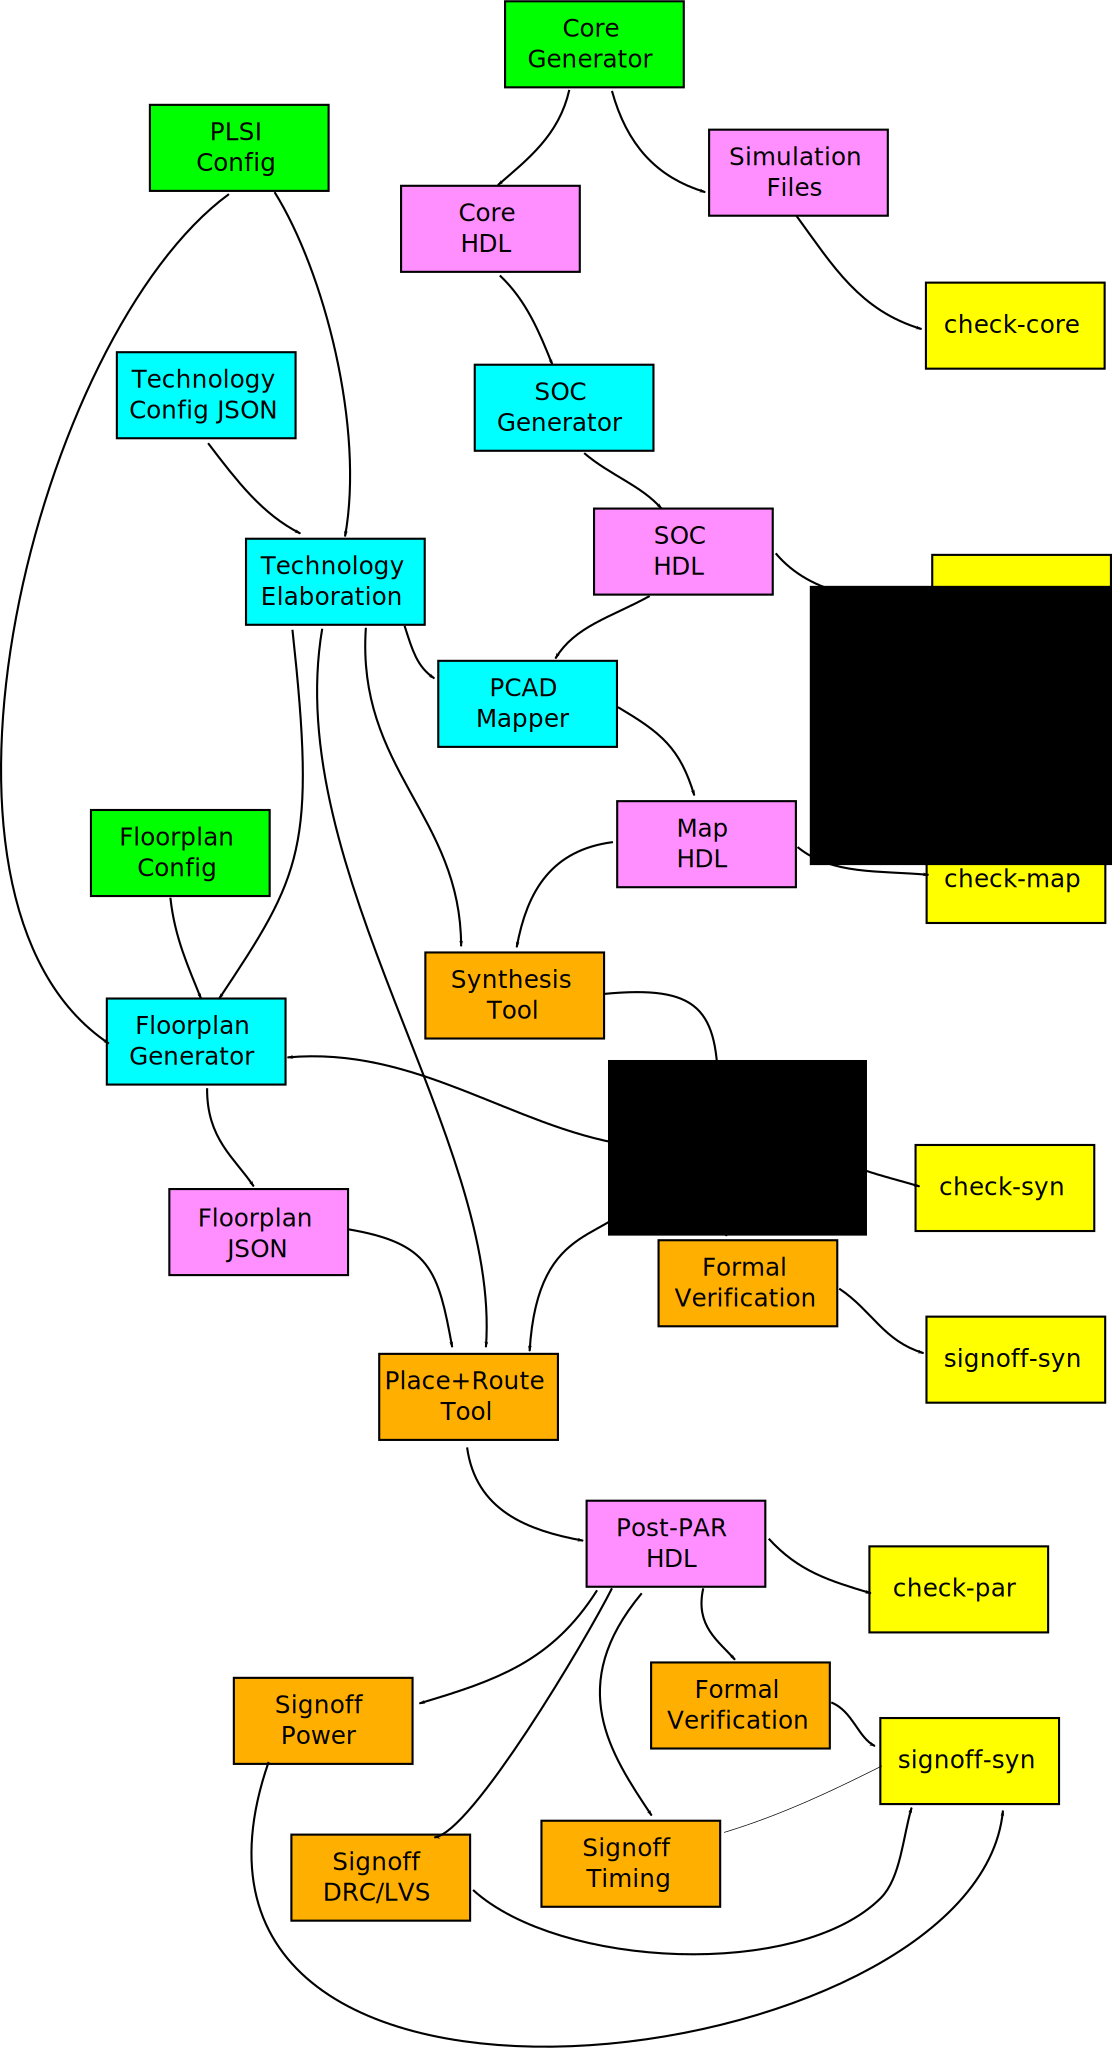
\includegraphics[width=0.7\linewidth]{figures/plsi-flow.svg}
\end{center}
\caption{A high-level overview of PLSI}
\label{impl:plsi-flow}
\end{figure}

\section{Core Generators}

PLSI was designed to support RTL-based research into microarchitectures by
quickly providing ground-truth power numbers for a large number of core
designs.  Thus the whole point of PLSI is that it is easy to port to new cores.
Porting PLSI to a new core generator based on Rocket Chip is extremely easy:
users simply need to point PLSI at their fork of Rocket Chip.  For example,
Figure~\ref{impl:hwacha-coregen} shows how little code is required to port PLSI
to the Hwacha vector unit.

\begin{figure}
\begin{verbatim}
CORE_DIR ?= $(CORE_GENERATOR_ADDON)/src/rocket-chip

RC_CORE_ADDONS = hwacha
CORE_TOP = ExampleTop

include src/addons/core-generator/rocketchip/vars.mk
\end{verbatim}
\caption{The core-generator addon for Hwacha}
\label{impl:hwacha-coregen}
\end{figure}

Porting PLSI to a core generator that isn't based on Rocket Chip is a bit more
involve.  The most interesting part of porting to PLSI is producing the list of
macros that the core requires.  There is a custom FIRRTL backend in PLSI that
allows Chisel based designs to easily generate PLSI macro configurations (this
tool is automatically used for Rocket Chip based projects), but Verilog based
cores have a bit more work to do.  I haven't actually managed to get a
reasonable open-source Verilog core, so I haven't ported PLSI to one yet.

\section{SOC Generators}

The SOC generation step converts a processor into an actual chip.  This means
inserting things like pads, clock recievers, etc.  For performing evaluations
of microarchitectures there is a ``nop'' SOC generator, which just doesn't do
anything.  This provides a simple way of evaluating a design without getting
into the complexities of chip building.  This was the only SOC generator used
for this thesis.

In addition to the ``nop'' SOC generator, there is also a ``bar-testchip'' SOC
generator.  This SOC generator generates a controller and phy that
transparently shims all top-level decoupled interfaces over a low-speed,
single-ended interface that is feasible to implement using the standard digital
IO pads that a popular commercial foundry provides.  This is designed to
provide a simple mechanism for building research-style test chips: it
alleviates the need to maintain chip-specific IO harnesses.  This SOC generator
was used to build a real chip on an agressive technology, but I've been removed
from the NDAs so I can't bring up the chip to see if it works or not.  The
process is completely automated: a PLSI tool reads to top-level Verilog of the
target design (using a Verilog parser I wrote), infers the decoupled
interfaces, generates an ASIC top-level wrapper and a test harness for both
FPGAs and simulation.

\section{Technology Mapping}

The technology mapping step converts generic macro implementations to those
that are specific to a particular technology.  This step is important to
maintaining portability of designs to multiple technologies: RTL writers should
never describe a technology-specific concept in their code but should instead
describe a generic version of that concept, which the mapping step then maps to
a technology-specific implementation.  This is really just a synthesis tool,
but it handles all the things that commercial synthesis tools don't understand.

The most important example of this is mapping sequential memories to SRAMs on
ASIC targets.  This is something that traditional synthesis tools can't do
because it's impossible to safely infer ASIC SRAMs from synthesizable Verilog.
Chisel and FIRRTL handle this mismatch by having an explicit memory visible to
the RTL programmer, which has been designed such that it can be mapped to ASIC
SRAMs.  PLSI uses this information to generate ASIC SRAM wrappers which can
then be passed on to the remainder of the CAD flow.

\subsection{Macro JSON Files}

PCAD has standardized on JSON as the interchange format between every step in
the flow because it's a well supported format.  The technology mapping step
expects a list of all the macros that need to be implemented and a list of all
the macros availiable to the technology.  Figure~\ref{impl:core-macro-list}
shows an example of one of the branch predictor memories in one of the BOOM
configurations, and Figure~\ref{impl:tech-macro-list} shows the ASIC SRAM that
will be used to implement that memory on the 32nm EDK.  

\begin{figure}
\begin{verbatim}
  {
    "type": "sram",
    "name": "h_table_ext",
    "depth": 32768,
    "width": 1,
    "ports": [
      {
        "clock port name": "RW0_clk",
        "mask granularity": 1,
        "output port name": "RW0_rdata",
        "input port name": "RW0_wdata",
        "address port name": "RW0_addr",
        "mask port name": "RW0_wmask",
        "chip enable port name": "RW0_en",
        "write enable port name": "RW0_wmode"
      }
    ]
  },
\end{verbatim}
  \caption{An example memory that needs to be mapped}
  \label{impl:core-macro-list}
\end{figure}

\begin{figure}
\begin{verbatim}
  {
    "family": "1rw",
    "width": 8,
    "name": "SRAM1RW1024x8",
    "ports": [
      {
        "write enable port name": "WEB",
        "clock port polarity": "positive edge",
        "output port polarity": "active high",
        "write enable port polarity": "active low",
        "address port polarity": "active high",
        "chip enable port polarity": "active low",
        "clock port name": "CE",
        "input port name": "I",
        "output port name": "O",
        "chip enable port name": "CSB",
        "read enable port name": "OEB",
        "input port polarity": "active high",
        "address port name": "A",
        "read enable port polarity": "active low"
      }
    ],
    "type": "sram",
    "depth": 1024
  },
\end{verbatim}
  \caption{An example ASIC SRAM macro description}
  \label{impl:tech-macro-list}
\end{figure}

\subsection{PCAD Macro Compiler}

In order to map technology-agnostic macros to technology-specific macros, I
implemented what is in effect a synthesis tool with a limited scope.  This tool
is an optimizing synthesis tool that uses some very simple optimization
techniques.  The only macro type I bother optimizing is the memories because
they're the only macros that I can compile that have any optimizations
potential.

\subsection{Technology JSON Files}

All the technology-specific information in PLSI is described within a single
file: the technology configuration file.  Defining all technology-specific
information in this manner is what allows 

\section{Synthesis Tool Driver}

\section{Place and Route Tool Driver}

\end{document}
